\documentclass[fontsize=9pt,paper=a5,fleqn,%parskip=full-,
DIV15,BCOR5.0mm,smallheadings,final, openany]{scrbook}
\usepackage{scrpage2}
\usepackage[OT1]{fontenc}
\usepackage[utf8]{inputenc}
%\usepackage{ngerman} 
\usepackage[ngerman]{babel}
%\usepackage{umlaute}
\usepackage{amsmath,amssymb}

%\usepackage{color}
\usepackage[final]{graphicx}
%\usepackage{url}
\usepackage{multicol}
\usepackage{polynom}
\usepackage{vorkurs}
\usepackage[breaklinks=true,pdftex,final,]{hyperref}
%\usepackage{url}
\usepackage{microtype}
%Programmierung
\usepackage{listings}

%\usepackage[Bjornstrup]{fncychap}
\setcounter{tocdepth}{0} % Nur Kapitel im Inhaltsverzeichnis anzeigen
\renewcommand*{\chapterheadstartvskip}{\vspace{0pt}} % Kein Leerraum ueber Ueberschrift
\setlength\mathindent{1pc} % Einzug von Mathe-Bloecken
\setcapindent{1em} % Einzug der zweiten Zeile in Unterschrift aendern
\automark[chapter]{chapter} % Kapitelname in Kopfzeile links und rechts 

%\includeonly{funktionen,trig,log_e}

\begin{document}

\title{Vorkurs Mathematik}
\author{Sebastian Mai \\ Kai Dannies
%FaRaFIN Vorkurs-Team
}
\publishers{\begin{center} \hspace*{1cm}\includegraphics%[viewport = 60 700 660 790]
{./images/farafin_logo_schwarz_auf_weiss.png}\end{center}}
\lowertitleback{Dieses Heft wurde vom Fachschaftsrat der Fakultät für
Informatik der Otto-von-Guericke-Universität Magdeburg für den
Mathematik-Vorkurs 2011 produziert.}
\date{2011}
\maketitle
\tableofcontents

\section {UNIX}

\subsection {Wozu sollte man lernen, wie man UNIX benutzt?}
Viele der Grundprinzipien von UNIX sind in heutigen Betriebssystem noch vorhanden und mit einigen dieser Betriebssysteme werdet ihr im laufe eures Studiums noch zu tun haben.

\subsection {Verzeichnisstruktur}
In Unix wird alles, egal ob es sich um eine Netzwerkschnittstelle, die Festplatte oder eine Musikdatei handelt als Datei repräsentiert. Alle diese Dateien lassen sich im sogenannten "Verzeichnissbaum" des Betriebssystems finden. Das wohl wichtigste Verzeichnis in UNIX ist "/" – das Wurzelverzeichnis. In diesem Verzeichnis liegen alle anderen Verzeichnisse.
An dieser Stelle lernen wir die ersten beiden Kommandos für das Terminal kennen: "ls" und "cd". Sie sind die wichtigsten Kommandos für die Navigation durch den Verzeichnissbaum von Unix. "cd" steht für "change directory" und lässt uns das Verzeichnis wechseln. Gibt man also "cd /" ins Terminal ein, so wechselt man ins Wurzelverzeichnis. "ls" steht für "list search", es liefert eine Auflistung der Dateien im aktuellen Ordner.
Da in Unix alles eine Datei ist, sieht man auch die Unterverzeichnisse des aktuellen Verzeichnisses.
Die Verzeichnisse im Wurzelverzeichnis sind bei den meisten Betriebssystemen (fast) gleich und jedes dieser Verzeichnisse erfüllt die selbe Bedeutung.

* / - das Wurzelverzeichnis
* /bin – Ausführbare Programme, z.B. die Shell /bin/sh 
* /boot - der Betriebssystemkern und was zum hochfahren benötigt wird
* /dev - "Devices" zum Beispiel Festplatten, USB-Geräte, der Zufallszahlengenerator ...
* /etc - Konfigurationsdateien für das Betriebssystem 
* /home - Das Elternverzeichnis aller Nutzerverzeichnisse
* /lib - Bibliotheken für andere Programme
* /opt - manuell installierte Programme
* /proc - Systemressourcen
* /root - Das Heimatverzeichnis des "root"-Nutzers
* /sbin - das "bin" für Programme die nur root ausführen darf
* /tmp - Temporäre Dateien
* /usr - "unix system resources" Datein die für alle Nutzer relevant sind
* /var - Variabel

Außerdem gibt es noch Kurzschreibweisen für bestimmte Verzeichnisse. "." beszeichnet das aktuelle Verzeichnis, ".." das Elternverzeichnis und "~" das eigene Homeverzeichnis.
Verzeichnisse die mit "." beginnen sind versteckt. Man kann sie anzeigen, wenn man ls mit dem Parameter "-a" benutzt.

\subsection {Arbeiten im Textmodus}
Unix stammt aus Zeiten, in denen man einen Rechner mit mehreren "Terminals" bedient hat. Ist man an so einem Terminal angemeldet, sieht man erstmal die Ausgabe des sog. "Command Line Interpreters" – /bin/sh. Dieses Programm ist im wesentlichen dafür zuständig, andere Programme aufzurufen. Hinter dem Kommando "ls" versteckt sich zum Beispiel ein Aufruf des Programms /bin/ls. Außerdem gibt es noch einige zusätzliche Kommandos, wie "help". Das wichtigste Kommando in Unix ist "man". Mit "man" lassen sich die sogenannten Manpages zu einem Programm anzeigen. In der Manpage stehen alle wichtigen Informationen, die man zu einem Programm braucht.
"man man" gibt zum Beispiel eine Hilfeseite zur Benutzung der Manpages aus.

\subsubsection {Wichtige Befehle}
* cat - gibt den Inhalt einer Datei aus
* cd - Verzeichnis wechseln
* cp - kopiert eine Datei
* date - zeigt das aktuelle Datum und die Uhrzeit an
* echo - gibt die Eingabe zurück
* exit - aktuelle Terminalsession beenden
* gedit - ruft einen Texteditor auf
* grep - Durchsuchen einer Datei
* javac - Javacompiler aufrufen
* java - ein Javaprogramm ausführen
* ls - zeigt den Inhalt des aktuellen Verzeichnisses
* man - zeigt eine Hilfeseite an
* mkdir - legt ein Verzeichnis an
* mv - verschiebt eine Datei
* passwd - eigenes Passwort ändern
* pwd - Zeigt das Verzeichnis an
* rm - Datei löschen
* ssh - eine Shell auf einem anderen Rechner öffnen
* tar - Dateiarchive packen und entpacken
* wget - herunterladen einer Datei
* yes - wiederholt die Eingabe

\subsubsection {Befehlssyntax}
Um einen Befehl richtig ausführen zu können benötigt dieser eine bestimmte Form. Ein typischer Unixbefehl könnte so aussehen:
"ls -lBh ~/". ls ist der ausgeführte Befehl, -l, -B und -h sind Parameter für das Programm ls und "~/" der Pfad zum Verzeichnis, dessen Datein ls auflisten soll. "~" ist eine abgekürzte Schreibweise für das eigene home-Verzeichnis.i
Genau so werden die Parameter und der richtige Aufruf von ls auch in der Manpage beschrieben. Mehrere Parameter können oftmals auch zusammengefasst werden, so dass "ls -l -a ..." die selbe Bedeutung hat wie "ls -la .."

\subsubsection {Befehle verknüpfen}
In Unix können auch mehrere Befehle verknüpft werden. Dazu gibt es mehrere nützliche Operatoren.
* & - "command &" führt das Kommando im Hintergrund aus
* && - mit "command1 && command2" kann man mehrere Kommandos hintereinander ausführen z.B. "mkdir foo && ls -l && cd foo/"
* | - mit "command1 | command2" kann man die Ausgabe von Kommando1 in Kommando2 verwenden  z.B. "ls -l | grep foo"

Man kann mit diesen Verknüpfungen aber auch sehr viel Schabernack treiben, man sollte davon nicht mehr benutzen als man benötigt, da man so unnötige Fehler vermeiden kann.
Weitere nützliche Operatoren sind:
* > - "command > file" schreibt die Ausgabe der Befehls in die angegebene Datei
* >> - wie ">", hängt die Ausgabe hinten an die Datei an

\subsubsection {Vom Textmodus zum Graphikmodus und wieder zurück}
Wie man zum Beispiel in den Rechnerpools der Fakultät sieht, besitzen moderne Unixoide Betriebssysteme nicht mehr ausschließlich den Textmodus. Man kann auch wie gewohnt in Fenstern bunte Bildchen anschauen.
Im Gegensatz zu Windows, kann man hier allerdings Programme nicht wirklich von der Shell losgelöst starten – die Ein- und Ausgaben sind nur für den User nicht mehr sichtbar. Besonders deutlich wird wenn man zum Beispiel "firefox" über ein Terminal startet – ob Webbrowser, Spiel oder Programmierumgebung – jedes Programm hängt an der Shell.
Die Wichtigkeit der Shell und für viele Entwickler der Grund überhaupt eine Shell zu benutzen heißt Secure Shell. Mit dem Befehl "ssh" kann man nämlich auch eine Shell auf einem anderen Unix-Rechner öffnen und sich Beispielsweise von Zuhause im Rechnerpool der FIN einloggen und dort arbeiten – sogar mit Programmen die man lokal gar nicht installiert hat. Mit "ssh -x" kann man sogar Graphikmodus-Programme benutzen.
Im Gegensatz zum Remotedesktop werden hier allerdings wesentlich weniger Daten übertragen und der Computer bleibt (einigermaßen) schnell.

\chapter{Die Grenzen eines Computers}

Der Computer kann eigentlich nur eine Sache: sehr schnell rechnen. Die Programme, die diese Fähigkeit ausnutzen lassen einen Computer oft sehr viel klüger erscheinen als er aussieht. Ein sehr berühmtes Programm, welches genau diese Tatsache demonstriert wurde in den 70er Jahren von Joseph Weizenbaum geschrieben: ELIZA. Es ist ein Programm, welches mit einem menschlichen Nutzer kommunizieren kann. Hier ein Beispiel davon:

\begin{itemize}
	\item[ELIZA:] Is something troubling you ?
	\item[YOU:] Yes, actually I try to setup an example with you.
	\item[ELIZA:] I understand.
	\item[YOU:] Can you help me with this?
	\item[ELIZA:] You like to think I help you -- don't you ?
	\item[YOU:] Yes I do.
	\item[ELIZA:] You say yes you do ?
	\item[YOU:] Yes I do.
	\item[ELIZA:] Do you say yes you do for some special reason ?
	\item[YOU:] Because I want you to help me.
	\item[ELIZA:] Suppose you got I to help you soon.
	\item[YOU:] I don't understand you.
	\item[ELIZA:] Does that trouble you ?
	\item[YOU:] Yes, a little bit
	\item[ELIZA:] You seem to be quite positive.
	\item[YOU:] You talk nonsense.
	\item[ELIZA:] Oh, I talk nonsense ?
	\item[YOU:] Yes you do.
	\item[ELIZA:] We were discussing you -- not me.
\end{itemize}

Unter \url{http://www.masswerk.at/elizabot/} kannst du es selber ausprobieren wenn ihr wollt. Auch dieses Programm zeigt keinerlei Intelligenz, obgleich die Antworten meistens Sinn machen. Der Computer macht nichts anderes als eine Antwort, basierend auf den Informationen die er in einer Datenbank hat, auszurechnen die wahrscheinlich eine sinnvolle Antwort auf die Aussage des Nutzers ist. Damit der Computer so etwas kann, musst du als Programmierer ihm beibringen, wie er mit simplen Rechenoperationen dieses Ergebnis erreicht.

\section{Arbeitsweise eines Rechners}

Ein Rechner versteht nur einen sehr begrenzten Satz von Befehlen. Diese Befehle sind zum Beispiel Laden von oder Speichern in eine Speicheradresse, Addieren von zwei Werten oder das Vergleichen von zwei Werten. Mit Hilfe solcher sehr einfachen Anweisungen müssen alle Programme geschrieben werden. Als ob das noch nicht schwer genug wäre, versteht der Rechner nur die Eingabe von Einsen und Nullen. 

\begin{itemize}
	\item[]1100 0000 0000 0000
	\item[]1001 1010 1011 1000
	\item[]1001 1010 1100 0000
	\item[]0000 0000 0000 0000
	\item[]0000 0000 0000 0000
	\item[]1001 1000 1100 0000
	\item[]1100 1111 1111 1011
\end{itemize}

Den obenstehenden Maschinencode kann ein Rechner lesen und interpretieren. Da dieser Code aber weder gut lesbar noch einfach zu schreiben ist, entwickelten Informatiker im Laufe der Jahre verschiedene Abstraktionen um das Programmieren einfacher zu machen.

Eine Abstraktionsebene ist Assembler. Ein Beispiel für ein Assemblerprogramm:

\begin{minipage}{\textwidth}
\begin{lstlisting}
ORG 100h 
push cs
pop ds 
mov ah, 09h
mov dx, Meldung 
int 21h
int 20h
 
Meldung: db "Hello World"
         db "$" 
\end{lstlisting}
\end{minipage}

Das Programm macht nichts außer einem ''Hello World'' auf der DOS-Konsole auszugeben. Das ist zwar besser lesbar als der Maschinencode aber immer noch nicht gut lesbar. Deshalb gibt es eine weitere Abstraktionsebene. Diese Abstraktionsebene sind die höheren Programmiersprachen wie C, C++, Java, Python und so weiter. Auf dieser Abstraktionsebene programmieren die meisten Programmierer. In diesem Vorkurs werden wir uns mit der Sprache Java beschäftigen.
\chapter {Hello World!}

\section {Wozu "Hello World!"?}

Fast alle Bücher, Tutorials, Vorkurshefte und sonstige Programmierbeispiele beginnen mit einem einfachen Programm, das nichts tut als "Hello World!" auf der Konsole auszugeben.

Im Grund behandelt man mit dem "Hello World!"-Programm zwei Fragen: 
* Was und an welchen Stellen kann ich im Quelltext ändern, um ein tolleres Programm zu erhalten?
* Wie komme ich von der Quelltext-Datei zum laufenden Programm?

In den meisten Programmiersprachen gibt es eine Art "Rahmen" der die eigentliche Programmlogik umgibt.
In Java sieht das Hello-World-Programm wie folgt aus: 
\begin{verbatim}
public class Hello {
  public static void main(String args[]) {
    System.out.println("Hello World!");	// gibt 'Hello World' aus.
  }
}
\end{verbatim}

Die erste Zeile enthält unter anderem den Namen des Programms nämlich "Hello". Die Datei mit dem Quelltext muss demzufolge "Hello.java" heißen.
"public static void main(String args[]) {" ist der Anfang der Main-Funktion des Programmes. Hier stehen die Befehle, die nach Programmstart als erstes abgearbeitet werden.
System.out.println("Hello World!"); – Das ist der Befehl der ausgeführt wird. "System.out.println" ist der Befehl der Text ausgibt, "Hello World!" der Text den wir ausgeben wollen. Die beiden Schließenden Klammern sind das Ende der Main-Funktion und das Ende des Programmes. 
Wenn wir also ein anderes Programm schreiben wollen, müssen wir lediglich den Befehl "System.out.println ..." durch andere Befehle ersetzen.

Um das Programm auszuführen, müssen wir zuerst den Quelltext des Programms in Bytecode umwandeln lassen und dann die Java-Virtual-Maschine aufrufen, die den Bytecode aufsführt. 
Für das Übersetzen des Quelltextes in Bytecode ist der Java-Compiler zuständig
Unter UNIX ruft man den Java-Compiler aus dem Terminal mit "javac Hello.java" auf. Der Compiler hat nun, sofern das Programm keine Fehler enthält eine Datei mit dem Namen "Hello.class" erzeugt (oder eine ältere Version überschrieben) – diese Datei enthält den Bytecode.
Die JVM kann man mit dem Befehl "java" aufrufen. "java Hello" führt den Bytecode in Hello.class aus.

%\include{Sequenz}
\chapter{Variablen und Datentypen}
Computerprogramme weisen im Wesentlichen drei relativ unabhängige Komponenten auf: Eingabe, Verarbeitung und Ausgabe. Bis jetzt haben wir uns nur mit der Ausgabe beschäftigt.
Die einfachste Form der Eingabe kennen wir auch schon: Wir setzen Werte im Quelltext. Ein Beispiel dafür ist unser „Hello World“-Proramm, indem wir festlegen das genau „Hello World“ und nicht „foobar“ ausgeben werden soll.
Um komplexere Eingaben, Verarbeitung und die Ausgabe dieser veränderlichen Daten zu ermöglichen brauchen wir eine Möglichkeit Daten abzuspeichern und zu bearbeiten, die vor dem Programmaufruf noch nicht bekannt sind.
Genau dies erlaubt das Konzept der Variablen. Eine Variable ist ein Platzhalter für einen dieser unbekannten Werte. \\

Ersetzen wir im „Hello World“-Programm die Zeile
\begin{lstlisting}
System.out.println("Hello World");
\end{lstlisting}
durch die folgenden drei Zeilen:
\begin{lstlisting}
String text; // legt eine Variable mit der Bezeichnung text an.
text = "Hello World"; // weist der Variable text den Wert "Hello World" zu.
System.out.println(text); // gibt den Wert der Variablen text aus.
\end{lstlisting}

Das neue Programm tut dasselbe wie das ursprüngliche „Hello World“-Proramm, ist allerding besser als das alte, denn die Ausgabe ist jetzt von der Eingabe (im Quelltext) getrennt.

\section {Befehle}
Wie wir sehen ist das „Hello World“-Programm länger geworden. Um Variablen zu manipulieren braucht man nämlich Befehle. Diese Befehle kann man daran erkennen, dass sie mit einem Semikolon enden. Abgearbeitet werden sie in der Reihenfolge in der man sie liest. Im Quelltext oben stehen drei Befehlsaufrufe:
Die Deklaration einer Variablen, eine Wertzuweisung und ein Funktionsaufruf. Das sind drei der wichtigsten Befehlsarten.

\subsection {Deklaration und Definition}
Um mit Variablen arbeiten zu können braucht man zwei Schritte: Deklaration und Definition.

„Sei p eine Primzahl” entspricht in etwa dem, was man dem Compiler bei der Deklaration einer Variable sagt. Um Werte digital abspeichern zu können muss man Wissen, um was für Daten es sich Handelt. Eine Zahl muss anders abgespeichtert werden, als zum Beispiel eine Zeichenkette wie „Hello World“.
Glücklicherweise müssen wir als Programmierer uns keine Gedanken mehr darum machen, wie die Daten intern repräsentiert werden.
Um auszudrücken um was für Daten es sich handelt gibt es sogenannte Datentypen. Eine kleine Auswahl der verfügbaren Typen findest du in der Tabelle.

todo: Tabelle mit Datentypen hier einfügen.

Der Befehl für die Definition einer Variablen sieht so aus: 
\begin{lstlisting}
Typname variablenname;
\end{lstlisting}
Beachtet, das Variablennamen üblicherweise kleingeschrieben werden.

Jetzt kennt der Compiler den Typ der Variablen. 
Damit man auch etwas mit Variablen anfangen kann braucht die Variable noch einen Wert – die Wertzuweisung heißt Definition der Variablen.
Eine Zuweisung sieht so aus: 
\begin{lstlisting}
variablenname = Wert;
\end{lstlisting}
Wichtig ist dabei vor allem eins: Das „=“ (der Zuweisungsoperator) hat eine (Lese-)Richtung. Der Wert den die Variable bekommt steht immer rechts!
Man kann in einer Zuweisung auch den (alten) Wert der Variable oder den einer anderen Variablen verwenden: \lstinline$p = 2 * p + q;$.

Außerdem gibt es noch zwei Kurzschriebweisen, die oft verwendet werden:
\begin{lstlisting}
x += y; // entspricht x = x + y;
        // Das funktioniert auch mit *=, /= und -=

x++; // entspricht x = x + 1;
x--; // x = x - 1;
\end{lstlisting}
Definition und Deklaration können auch in einer Anweisung gemacht werden: 
\begin{lstlisting}
String text = "Hello World";
\end{lstlisting}
Beachtet, das der Datentyp von Rechter und Linker Seite der Zuweisung übereinstimmen müssen. Es kann allerdings auch sein, dass ihr das gar nicht wollt.
Um den Typ einer Variablen zu ändern gibt es sogenannte Casts. Integrale Datentypen wie int oder char könnt ihr ineinander umwandeln, indem ihr den eingeklammerten Namen des Zieldatentyps vor die Variable schreibt: 
\begin{lstlisting}
char c = (char) intvariable;
\end{lstlisting}
Das \lstinline$(char)$ sorgt dann dafür, dass aus der Ganzzahl ein Buchstabe gemacht wird.
Für andere Typänderungen gibt es Funktionen.

\subsection{Funktionsaufrufe}
Funktionen sind vorgefertigte Unterprogramme, die einen bestimmten Zweck erfüllen. Eine Funktion kennt ihr schon: \lstinline$System.out.println()$.
Diese Funktion tut etwas, und gibt dann die Kontrolle wieder an den nächsten Befehl ab. Es gibt aber auch Funktionen, die einen Wert berechnen.
Diesen Wert nennt man Rückgabewert. Die Funktion \lstinline$Math.random()$ hat als Rückgabewert einen zufälligen Wert.
Wie packt man nun Funktionen in einen Befehl? Interessiert uns der Rückgabewert der Funktion, so benutzen wir die Funktion in einer Zuweisung: 
\begin{lstlisting}
zufallszahl = Math.random();
\end{lstlisting}
Interessiert uns der Rückgabewert nicht, so lassen wir die linke Seite der Zuweisung einfach weg:
\begin{lstlisting}
Math.random();
\end{lstlisting}
Viele Funktionen, beispielsweise \lstinline$System.out.println()$, sind in der Lage Daten weiterzuverarbeiten. Dafür muss der Funktion allerdings mitgeteilt werden, welche Daten gemeint sind.
Um diese Daten an die Funktion zu übergeben gibt es die Klammern nach dem Funktionsnamen. Dort kann man die entsprechenden Werte eintragen.
Sollen der Funktion mehrere Werte übergeben werden, so müssen diese durch Kommata getrennt werden – die Reihenfolge der Parameter entscheidet dabei darüber, welcher Wert wofür benutzt wird.
\begin{lstlisting}
funktion(parameter1, parameter2 /* . . . */);
\end{lstlisting}

\section {Einlesen von Werten}
Um Werte einzulesen braucht man einen Variable vom Typ \lstinline$Scanner$. Mit dem Scanner kann man nicht nur von der Standarteingabe, sondern auch aus Dateien, Netzwerkverbindungen und anderen Quellen Daten einlesen. 
Deswegen muss man Angeben, dass der Scanner die Daten aus \lstinline$System.in$ beziehen soll.
Danach kann man mit \lstinline$scannervariable.next()$ die nächste Eingabe abholen. Im Quelltext könnte das zum Beispiel so aussehen:
\begin{lstlisting}
import java.io.*;
import java.util.Scanner;

public class Hello {
	public static void main(String args[]) {
		Scanner scanner;	// Beachtet den unterschied zwischen Datentyp('S') und Variable('s')!
		scanner = new Scanner(System.in); // Legt einen Scanner an, der System.in ueberwacht
		String name = scanner.next();
		System.out.println("Hello " + name + "!");
	}
}
\end{lstlisting}
Damit ist unser „Hello World“-Programm, schon richtig gut, denn es kann nun auf Nutzereingaben reagieren.

\section {Aufgaben}
\begin{itemize}
\item Sieh der das neue Programm "Hello.java" an.
\item Füge eine neue Textausgabe ein, die den Nutzer auffordert seinen Namen einzugeben, sonst weiß er nicht, dass er etwas eingeben soll.
\item Schreibe ein Java Programm, dass den Ape-Faktor einer Person ausgibt, nachdem man Größe und Armspanne eingegeben hat. (Der Ape-Faktor ist die Differenz zwischen Größe und Armspanne einer Person)
\item Schreibe ein Programm, dass den ASCII-Code eines eingegeben Buchstaben ausgibt.
\end{itemize}

Zusatz: Schreibe ein Programm, dass einen Buchstaben mit der Caesar-Verschlüsselung (mit Variabler Verschiebeweite) verschlüsseln kann.

\chapter{Schleifen und Arrays}

\section{Schleifen}

Mit dem bisher gelernten Wissen sollte folgende Aufgabe für dich leicht zu lösen sein: Schreibe ein Programm, das die Zahlen von 1 bis 12 ausgibt. Etwas schwieriger wird die Aufgabe, wenn du die Zahlen von 1 bis einer Million ausgeben sollst oder die Obergrenze von einer Nutzereingabe abhängt. An dieser Stelle kommen Schleifen ins Spiel: Sie führen einen Anweisungsblock solange aus, bis eine bestimmte Bedingung erfüllt (oder nicht mehr erfüllt) ist. Java kennt, wie viele andere Programmiersprachen auch drei verschiedene Arten von Schleifen: Die \textit{for}-Schleife, die \textit{while}-Schleife und die \textit{do-while}-Schleife.

\subsection{Die FOR-Schleife}

Diese Schleife ist die, die man vermutlich am häufigsten sieht. Im Struktogramm wird sie wie in Abbildung \ref{for} verwendet.

\begin{figure}
	\begin{center}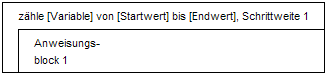
\includegraphics[scale=1]{images/for.png}\end{center}
	\caption{Die \textit{for}-Schleife in einem Struktogramm}
	\label{for}
\end{figure}

Für diese Art von Schleife braucht man eine explizite Laufvariable, die man inkrementieren kann. Im einfachsten Fall kann man dafür einen Integer benutzen. Das untenstehende Codebeispiel verdeutlicht die Benutzung einer \textit{for}-Schleife in Java.

\begin{minipage}{\textwidth}
\begin{lstlisting}
public class ForSchleife {
  public static void main(String[] args) {
    for(int i = 1; i <= 12; i=i+1){
      System.out.println(i);
    }
  }
}
\end{lstlisting}
\end{minipage}

Eine \textit{for}-Schleife braucht drei Informationen über die Laufvariable: Ihren Initialwert, hier mit \textit{int i = 1} geschehen, einen bool'schen Ausdruck wann die Schleife abbrechen soll, hier mit $i <=12$ angegeben. Das bedeutet, dass die Schleife nicht mehr ausgeführt wird, sobald $i$ diese Bedingung nicht mehr erfüllt, also 13 erreicht.

Am Ende benötigt man noch eine Aktion, die nach jedem Schleifendurchlauf gemacht werden soll, in diesem Fall wird mit \textit{i=i+1} die Laufvariable nach jedem Schleifendurchlauf inkrementiert.

\subsection{Die WHILE-Schleife}

Der Unterschied zu der \textit{for}-Schleife ist im Wesentlichen, dass keine konkrete Initialisierung benötigt und auf eine Behandlung der Variable nach jedem Schleifendurchlauf verzichtet wird. Im Struktogramm hat die \textit{while}-Schleife auch eine eigene Abbildung (\ref{while}).

\begin{figure}
	\begin{center}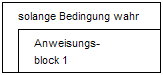
\includegraphics[scale=1]{images/while.png}\end{center}
	\caption{Eine \textit{while}-Schleife in einem Struktogramm}
	\label{while}
\end{figure}

In Java definiert der folgende Code eine \textit{while}-Schleife:

\begin{minipage}{\textwidth}
\begin{lstlisting}
public class IfThenElse {
  public static void main(String[] args) {
    int i = 1;
    while(i<=12){
      System.out.println(i);
      i = i+1;
    }
  }
}
\end{lstlisting}
\end{minipage}

Der Code hat den gleichen Effekt wie der bei der im letzten Abschnitt gezeigten \textit{for}-Schleife. Die Initialisierung findet hier jedoch vor der Schleife statt; die Inkrementierung der Variable findet in der Schleife statt.

\subsection{Die DO-WHILE Schleife}

Diese Schleife unterscheidet sich nicht wesentlich von der \textit{while}-Schleife. Im Gegensatz zu dieser wird die Bedingung aber erst am Ende geprüft und nicht am Anfang. Auch diese Schleife hat eine Entsprechung in einem Struktogramm (Abbildung \ref{dowhile}.

\begin{figure}
	\begin{center}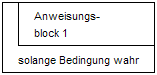
\includegraphics{images/dowhile.png}\end{center}
	\caption{Die \textit{do-while}-Schleife in einem Struktogramm}
	\label{dowhile}
\end{figure}

Der Javacode ähnelt ebenfalls sehr der \textit{while}-Schleife:

\begin{minipage}{\textwidth}
\begin{lstlisting}
public class IfThenElse {
  public static void main(String[] args) {
    int i = 1;
    do{
      System.out.println(i);
      i = i+1;
    }while(i<=12);
  }
}
\end{lstlisting}
\end{minipage}

Diese Schleife läuft also, unabhängig davon ob die Bedingung am Anfang erfüllt ist oder nicht, mindestens ein mal durch.

\subsection{Gefahren von Schleifen}

Jeder Code, den du bisher geschrieben hast, läuft bei korrekter Syntax durch und das Programm wird irgendwann beendet sein. Bei Schleifen ist diese Tatsache nicht mehr garantiert. Der folgende Code hat zwar eine völlig korrekte Syntax, wird aber bei der Ausführung eine niemals terminierende Endlosschleife sein:

\begin{minipage}{\textwidth}
\begin{lstlisting}
public class IfThenElse {
  public static void main(String[] args) {
    int i = 1;
    while(i<=12){
      System.out.println(i);
    }
  }
}
\end{lstlisting}
\end{minipage}

Hier wurde vergessen, die Variable, die in der Bedingung geprüft wird, zu ändern. Die Bedingung \textit{$i\le 12$} wird damit immer wahr sein und damit wird die Schleife nie verlassen. Wenn ihr also ein Programm schreibt, es laufen lasst und es hört einfach nicht auf zu rechnen, dann ist es möglicherweise solche eine Endlosschleife die das Problem erzeugt. Es ist eure Aufgabe als Programmierer, darauf zu achten das jede Schleife terminiert.

Im letzten Kapitel hast du bereits das Schlüsselwort \textit{break;} kennengelernt. Es wurde dazu verwendet um sofort aus einer \textit{switch}-Anweisung herauszuspringen. Ein \textit{break;} in einer Schleife hat die gleiche Funktion: Die Ausführung der Schleife wird sofort beendet und der Code wird nach der Schleife fortgesetzt.

\begin{minipage}{\textwidth}
\begin{lstlisting}
public class IfThenElse {
  public static void main(String[] args) {
    for (int i = 1; i <= 12; i++){
      System.out.println(i);
      if (i==6){
        break;
      }
    }
    System.out.println("Nach der Schleife");
  }
}
\end{lstlisting}
\end{minipage}

Das Ergebnis des obenstehenden Codes ist, dass nur die Zahlen von eins bis sechs ausgegeben werden und die Schleife danach mittels des \textit{break;} verlassen wird, unabhängig von dem Wahrheitswert der Abbruchbedingung der Schleife. 

Für Schleifen gibt es noch ein zweites derartiges Schlüsselwort: \textit{continue;}. Im Gegensatz zu \textit{break;} bricht es nicht die komplette Schleife ab sondern lediglich den aktuellen Schleifendurchlauf. Der untenstehende Code wird also alle Zahlen zwischen eins und zwölf ausgeben außer der 6:

\begin{minipage}{\textwidth}
\begin{lstlisting}
public class IfThenElse {
  public static void main(String[] args) {
    for (int i = 1; i <= 12; i++){
      if (i==6){
        continue;
      }
      System.out.println(i);
    }
    System.out.println("Nach der Schleife");
  }
}
\end{lstlisting}
\end{minipage}

\subsection{Aufgaben}

\begin{enumerate}
	\item Implementiere eine Schleife, die eine Integer-Zahl von der Konsole liest und alle natürlichen Zahlen kleiner oder gleich der gelesenen Zahl ausgibt. Implementiere das Programm mit Hilfe einer
	\begin{itemize}
		\item \textit{for}-Schleife
		\item \textit{while}-Schleife
		\item \textit{do-while}-Schleife
	\end{itemize}
	\item Verändere das Programm mit der \textit{for}-Schleife, sodass es nur noch die geraden Zahlen ausgibt. Verändere dabei
	\begin{itemize}
		\item nur den Anweisungsblock in der Schleife.
		\item nur den Schleifenkopf.
	\end{itemize}
	\item Schreibe ein Programm das von der Konsole zwei Integer $n$ und $m$ liest. Gib alle Zahlen zwischen $1$ und $n\cdot m$ in n Spalten und m Zeilen ausgibt. (Hinweis: Es ist möglich eine Schleife in einer Schleife zu definieren)
	\item Schreibe ein Programm das für eine eingegebene Zahl prüft, ob sie eine Primzahl ist. (Hinweis: Das Sieb des Eratosthenes bietet einen möglichen Algorithmus)
	\item Schreibe ein Programm welches alle Primzahlen bis zu einer von dem Nutzer eingegebenen Obergrenze ausgibt.
\end{enumerate}

\section{Arrays}

Du weißt bereits was Variablen und Datentypen sind. Wenn man beispielsweise die Höchsttemperatur eines Tages speichern möchte, kann man sich dafür ein \textit{double} deklarieren, in dem man diesen Wert speichern kann. Jetzt könnte man zum Beispiel die Aufgabe bekommen, die Höchsttemperaturen von jedem Tag der Woche zu speichern. Man kann dafür natürlich 7 Variablen anlegen. Wenn man den Zeitraum für das Speichern der Temperaturen aber ausweitet, zum Beispiel auf ein Jahr, dann kann auch das anstrengend werden.

Arrays sind ein Weg um die Speicherung solcher gleichartigen Datenmengen einfach umzusetzen. Man kann sich ein Array wie eine lange Reihe von Schließfächern vorstellen: in jedem Schließfach gibt es einen Inhalt, und mit der Nummer des Schließfachs kann man auf den Inhalt zugreifen. Die Verwendung von Arrays in Java zeigt das folgende Codebeispiel:

\begin{minipage}{\textwidth}
\begin{lstlisting}
public class IfThenElse {
  public static void main(String[] args) {
    double[] temperature = new double[365];
    temperature[42] = 13.37;
    System.out.println(temperature[42]);
    System.out.println(temperature[23]);
  }
}
\end{lstlisting}	
\end{minipage}

In der ersten Zeile wird der Container deklariert: Es wird Platz für 365 \textit{double}-Werte reserviert und jeder der Werte wird mit einem Standardwert, in diesem Fall $0.0$, initialisiert. In der zweiten Zeile befülle ich den 42. Platz des Containers mit einem Wert: $13.37$, der in der dritten Zeile wieder ausgegeben wird. Die Ausgabe in der vierten Zeile wird $0.0$ ausgeben, da kein anderer Wert diesem Container zugewiesen wurde.

\begin{itemize}
	\item[\textit{Bemerkung:}] Die Initialisierung mit einem Standardwert ist eine Eigenheit von Java. Viele andere Programmiersprachen, zum Beispiel C++, würden an dieser Stelle einen (mehr oder weniger) zufälligen Wert zurückgeben.
\end{itemize}

Ähnlich wie das Schachteln von Schleifen, können auch Arrays ''geschachtelt'' werden. Wenn man sich ein eindimensionales Array als Reihe eines Schachbretts vorstellt, dann ist das komplette Brett ein zweidimensionales Array. Ein dreidimensionales Array kann man sich als viele Schachbretter übereinander vorstellen. Die Vorstellung von Dimensionen größer als drei überlasse ich an der Stelle lieber den Mathematikern. Die Deklaration eines mehrdimensionalen Arrays kann wie folgt aussehen:

\begin{minipage}{\textwidth}
\begin{lstlisting}
public class IfThenElse {
  public static void main(String[] args) {
    String[][] chessBoard = new String[8][8];
  }
}
\end{lstlisting}	
\end{minipage}

Natürlich muss man auch bei Arrays auf Dinge achten. So kann man in Java bei einem Array, das mit $n$ Feldern initialisiert wurde auf die Felder $0$ bis $n-1$ zugreifen. Ein Zugriff auf einen Wert außerhalb dieses Bereichs führt zu einem Absturz des geschriebenen Programms. Ein weiterer Nachteil von Arrays ist es, dass man eine Größe beim Programm spezifizieren muss. Datenstrukturen, die diesen Nachteil umgehen wirst du im Laufe des ersten Semesters kennenlernen.

Eine häufig genutzte Funktion von Arrays ist das bestimmen der Größe um zum Beispiel die Anzahl der Schleifendurchläufe zu bestimmen:

\begin{minipage}{\textwidth}
\begin{lstlisting}
public class IfThenElse {
  private const int ARRAY_SIZE = 8;
  public static void main(String[] args) {
    int[] example = new int[ARRAY_SIZE];
    for (int i = 0; i < example.length; i++{
      //do something
    }
  }
}
\end{lstlisting}	
\end{minipage}

Insbesondere beim Einlesen der Größe des Arrays, wenn man also die Größe des Arrays nicht von vornherein kennt, ist diese Funktion sehr hilfreich.

\subsection{Aufgaben}

\begin{enumerate}
	\item Schreib ein Programm, das für ein Array von Integern oder Floats die Summe aller ihrer Elemente ausgibt.
	\item Schreib ein Programm, welches zwei gleich große Arrays von Integern oder Floats entgegennimmt und die Elementweise Summe in ein neues Array schreibt.
	\item Schreib ein Programm, welches die Größe eines zu erstellenden Arrays vom Nutzer einliest. Fülle dieses Array der Größe $n$ mit den ersten $n$ Primzahlen.
	\item Spieglein, Spieglein in meinem Programm, spiegle ein Zweidimensionales Array. (Es sollen sich also die Werte an anderen Stellen wiederfinden.
	\item Schreib ein Programm, in dem zu jeder Person mehrere schlechte Wortwitze abgespeichert werden können. Was wäre eine Wortspielkasse, ohne ein tolles Javaprogamm?
\end{enumerate}


\include{IdeeZuProgram}
\chapter{Funktionen}

Bislang sahen alle deine Programme folgendermaßen aus:

\begin{minipage}{\textwidth}
\begin{lstlisting}
public class Funktionen {
  public static void main(String[] args) {
    //do something
  }
}
\end{lstlisting}
\end{minipage}

Auch hier hast du schon eine Funktion verwendet, möglicherweise ohne es zu wissen: \textit{public static void main(String[] args)} definiert eine Funktion. Diese spezielle Funktion ist eine besondere: Sie deklariert für den Rechner den Einstiegspunkt in unser geschriebenes Programm. Euer Code wird beginnend in dieser Funktion ausgeführt. Ihr habt auch die Möglichkeit weitere Funktionen zu schreiben. Der Syntax dafür ist der folgende:

\begin{minipage}{\textwidth}
\begin{lstlisting}
public class Funktionen {
  public static void myFunction() {
    //do something
  }
}
\end{lstlisting}
\end{minipage}

Das erste Wort, \textit{public} ist ein Schlüsselwort, welches angibt wer diese Funktion benutzen kann. Ich möchte an dieser Stelle nicht in die Tiefe gehen, aber euch die möglichen Schlüsselwörter nicht vorenthalten:

\begin{itemize}
	\item \textit{public}
	\item \textit{private}
	\item \textit{protected}
\end{itemize}

Das zweite Schlüsselwort, \textit{static} sei für den Moment verpflichtend. Wenn ihr euch mit Objektorientierung beschäftigt, kann dieses Schlüsselwort ausgelassen werden. Das liegt aber außerhalb des Rahmen dieses Vorkurses.

Das dritte Schlüsselwort, \textit{void}, bezeichnet den Rückgabetyp einer Funktion. \textit{void} bedeutet dabei, dass diese Funktion keinen Rückgabetyp hat. Jede beliebige Bezeichnung eines Datentyps, zum Beispiel \textit{int, bool, String, ...} kann an dieser Stelle stehen. Wenn dort ein Datentyp stehen, muss diese Funktion einen Wert dieses Datentyps zurückgeben:

\begin{minipage}{\textwidth}
\begin{lstlisting}
public class Funktionen {
  public static int myFunction() {
    int someInt = 0;
    //do something
    return someInt;
  }
}
\end{lstlisting}
\end{minipage}

Das Schlüsselwort für das Zurückgeben eines Wertes ist \textit{return}. Wenn die Funktion \textit{return} erreicht hat, wird kein weiterer Code in der Funktion ausgeführt sondern sofort zurück in aufrufende Funktion gesprungen. In diesem Sinne funktioniert \textit{return} wie ein \textit{break}.

Diese Funktionen können nun genauso mit Code befüllt werden wie ihr bisher die \textit{main}-Funktion getan habt. Ein Beispiel ist das Folgende:

\begin{minipage}{\textwidth}
\begin{lstlisting}
public class Funktionen{
  //hier startet das Programm
  public static void main(String[] args){
    int number = readNumberFromConsole();
    bool isPrime = checkPrime(number);
    print(number, isPrime);
  }      
  
  public static int readNumberFromConsole(){
    int number;
    //you already should know the code for this
    return number;
  }
  
  public static bool checkPrime(int number){
    bool result;
    //you shall figure out this code for yourself
    return result;
  }
  
  public static void print(int number, bool isPrime){
    if(isPrime)
      System.out.println(number + " ist eine Primzahl");
    else
      System.out.println(number + " ist keine Primzahl");
  }
}
\end{lstlisting}
\end{minipage}

Das obenstehende Beispiel demonstriert die Verwendung von Funktionen. Manche Funktionen können Parameter besitzen, also Werte von denen diese Funktion abhängt. Bei der Definition einer Funktion werden diese benötigten Werte in den Klammern definiert. Unsere Funktion \textit{print} hängt beispielsweise von 2 Parametern ab: Einem \textit{int} und einem \textit{bool}.

Eine Funktion wird immer mit ihrem Namen und einer öffnenden und schließenden Klammer hinter dem Namen aufgerufen. In diese Klammern müssen konkrete Werte für alle Parameter, die diese Funktion benötigt übergeben werden. Wenn die Funktion keine Parameter besitzt bleiben diese Klammern leer.

Wenn Funktionen Werte zurückgeben, kann man diese Werte Variablen zuweisen oder andere Funktionen damit ''füttern'', wie im folgenden Beispiel:

\begin{minipage}{\textwidth}
\begin{lstlisting}
public class Functions{
  //hier startet das Programm
  public static void main(String[] args){
    int number = readNumberFromConsole();
    print(number, checkPrime(number));
  }      
  
  public static int readNumberFromConsole(){
    int number;
    //you already should know the code for this
    return number;
  }
  
  public static bool checkPrime(int number){
    bool result;
    //you shall figure out this code for yourself
    return result;
  }
  
  public static void print(int number, bool isPrime){
    if(isPrime)
      System.out.println(number + " ist eine Primzahl");
    else
      System.out.println(number + " ist keine Primzahl");
  }
}
\end{lstlisting}
\end{minipage}

\section{Exkurs: Rekursion}

Ein sehr beliebtes Zitat für Rekursion ist: ''Um Rekursion zu verstehen, muss man Rekursion verstanden haben''. Das trifft das Problem an der Rekursion ziemlich gut. Es ist eigentlich keine schwierige Sache, aber das menschliche Gehirn ist diese Art von denken nicht gewohnt. 

\begin{figure}
	\begin{center}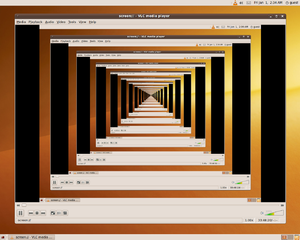
\includegraphics{images/rekursion.png}\end{center}
	\caption{Grafische Rekursion}
\end{figure}

Rekursion bedeutet, dass sich eine Funktion immer wieder selbst aufruft. Um eine sich wiederholende Struktur auszunutzen. Ein einfaches Beispiel dafür ist die Fakultät einer Zahl, wo bereits die Definition rekursiv ist:

\begin{center}
	$1! = 1$
	$n! = n\cdot (n-1)!$
\end{center}

Wie du siehst, wird die Fakultät benutzt um die Fakultät zu definieren. Die Rekursion hat außerdem noch eine Abbruchbedingung, in diesem Fall wenn $n=1$. Wenn ihr eine Rekursion programmiert, müsst ihr auch eine Abbruchbedingung programmieren. Der untenstehende Code ist ein Beispiel für die Fakultät die mit Hilfe von Rekursion gelöst wird.

\begin{minipage}{\textwidth}
\begin{lstlisting}
public class Rekursion{
  public static void main(String[] args){
    long number = 12;
    long result = factorial(number);
    System.out.println(result);
  }
  
  public static long factorial(long number){
    //Abbruchbedingung
    if(number <= 1){
      return 1;
    }
    //rekursiver Aufruf
    return number*factorial(number-1);
  }
}
\end{lstlisting}
\end{minipage}

In der Funktion \textit{factorial} findet ihr beide Elemente, die jede Rekursion enthalten muss. Zum Einen die Abbruchbedingung bei der geprüft wird, ob die Zahl kleiner als 2 ist. Wenn das so ist wird eine Konstante zurückgegeben. Zum Anderen findet ihr den rekursiven Aufruf, bei dem in der \textit{return}-Zeile wieder die Funktion aufgerufen wird.

\section{Aufgaben}

\begin{enumerate}
	\item Du kennst sicherlich den Bereich in diversen Supermärkten in denen die Einkaufswagen stehen. Mit dem Programm ShoppingCart.java wollen wir diesen Bereich jetzt nachbauen.
	\begin{itemize}
		\item Mach aus der Ausgabe eine Funktion mit einem aussagekräftigen Namen.
		\item Schreibe eine Funktion, die einen Einkaufswagen aus einer zufällig gewählten Reihe wegnimmt.
		\item Schreibe eine Funktion, die einen Einkaufswagen in eine zufällge Reihe einfügt.
		\item Schreibe eine Funktion, die den Einkaufswagen in der längsten Reihe wieder einreiht.
		\item Simuliere den Supermarkt in mehreren Schritten. Wenn du es dir leicht machen willst, nimmt der Kunde den Einkaufswagen in einer Phase mit und bringt ihn sofort zurück. Die Fortgeschrittenen Java-Programmierer unter euch können mehrere Kunden im Markt simulieren.
	\end{itemize}
	\item Schreibe ein Programm, dass die n-te Fibonaccizahl ausrechnet.
	\item Schreibe ein Programm, dass die Ackermannfunktion berechnet.
	\item Schreibe ein Programm, das die Fakultät berechnet ohne Rekursion zu benutzen.
\end{enumerate}

\chapter{Guter Programmierstil}

Oder: Wie schreibe ich meinen Code, sodass ihn auch andere lesen können?

''Guter'' Code ist unter Programmierern immer ein beliebtes Streitthema, weil jeder dort seine eigene Definition von gutem Code hat. Es gibt also keine allgemeingültigen Regeln, die man bei Code zu beachten hat. Trotzdem gibt es einige Dinge, die man auf jeden Fall machen sollte. Um die Wichtigkeit von sauberem Code zu erkennen, möchte ich zunächst mal die Unterschiede in der Lesbarkeit demonstrieren:

\begin{minipage}{\textwidth}
\begin{lstlisting}
public class A{public static void main(String[] args)
{int a=2;int b=3;int c=1;for(int i=0;i<b;i++){c=c*a;}
System.out.println(c);}}
\end{lstlisting}
\end{minipage}

Obenstehend ist ein Beispiel ohne jede Formatierung. Der gesamte Code steht einfach in einer Zeile (für die Lesbarkeit habe ich trotzdem Zeilenumbrüche hinzugefügt). Dieser Code würde so kompiliert und mit dem korrekten Ergebnis ausgeführt werden. Probiert einfach mal herauszubekommen, was dieser Code macht.

\begin{minipage}{\textwidth}
\begin{lstlisting}
public class A{
public static void main(String[] args){
int a=2;
int b=3;
int c=1;
for(int i=0;i<b;i++){
c=c*a;
}
System.out.println(c);
}
}
\end{lstlisting}
\end{minipage}

Dieser Code demonstriert eine der ersten Grundsätze: Jede Anweisung kommt in eine einzelne Zeile. Es erhöht die Übersicht enorm und der Code ist schon viel einfacher zu lesen. Aber es geht natürlich noch besser.

\begin{minipage}{\textwidth}
\begin{lstlisting}
public class A{
  public static void main(String[] args){
    int a=2;
    int b=3;
    int c=1;
    for(int i=0;i<b;i++){
      c=c*a;
    }
    System.out.println(c);
  }
}
\end{lstlisting}
\end{minipage}

Dieser Code enthält Einrückungen. Diese Einrückungen demonstrieren einen zusammenhängenden Codeblock. Insbesondere bei mehreren und komplexeren Funktionen hilft dies enorm um auf einen Blick mitzubekommen, welcher Code in welche Funktion / Schleife / Verzweigung gehört.

\begin{minipage}{\textwidth}
\begin{lstlisting}
public class Potenzieren{
  public static void main(String[] args){
    int basis=2;
    int exponent=3;
    int ergebnis=1;
    for(int i=0;i<exponent;i++){
      ergebnis=ergebnis*basis;
    }
    System.out.println(ergebnis);
  }
}
\end{lstlisting}
\end{minipage}

Im obenstehenden Code habe ich (fast) alle Namen die ich ersetzen kann ersetzt. Jede Variable, jeder Funktionsname und jeder Klassenname sollte widerspiegeln wozu die jeweilige Entität da ist. Eine Ausnahme ist auch im obenstehenden Beispiel zu erkennen: Zählvariablen in Schleifen werden in der Regel mit \textit{i, j, k} usw. benannt. Bei diesem Code kann man sehr leicht erkennen, was gemacht wurde weil man drei einfach Regeln beachtet hat:

\begin{itemize}
	\item jede Anweisung kommt in eine eigene Zeile
	\item jeder Inhalt zwischen zwei geschweiften Klammern wird eingerückt
	\item jeder Name den ihr wählen könnt soll einen Aussagekräftigen Namen bekommen
\end{itemize}

\section{Kommentierung}

Kommentierung ist den meisten Programmierern ebenfalls ein lästiges Thema. Aber auch hier gilt wieder: Gute Kommentierung macht den Code lesbarer. Die Kommentierung von Code findet auf drei Ebenen statt:

\begin{itemize}
	\item auf Klassenebene
	\item auf Funktionsebene
	\item auf Anweisungsebene im Code
\end{itemize}

Auf allen drei Ebenen erfüllen die Kommentare unterschiedliche Aufgaben. Auf Klassenebene wird die Frage ''Was macht diese Klasse?'' beantwortet. Auf Funktionsebene wird die Frage ''Wie wird die Aufgabe in der Funktion gelöst?'' beantwortet. Auf Anweisungsebene erklärt ein Kommentar, warum genau diese Anweisung durchgeführt wird. Als Faustregel gilt: wenn ihr vor eine Funktion oder eine Anweisung schreiben müsst, was dort passiert ist, dann habt ihr die Funktion oder die verwendeten Variablen nicht gut benannt. Ein Beispiel für Kommentierung:

\begin{minipage}{\textwidth}
\begin{lstlisting}
/*
 * Diese Klasse potenziert zwei Integer und gibt das 
 * Ergebnis auf der Konsole aus.
 */
public class Potenzieren{

  /*
   * Die Funktion fuehrt das Potenzieren aus, indem sie 
   * die Basis mehrfach in einer Schleife multipliziert
   */
  public static void main(String[] args){
    int basis=2;
    int exponent=3;
    //Das Ergebnis wird mit 1 initialisiert, weil x^0=1
    int ergebnis=1;
    for(int i=0;i<exponent;i++){
      ergebnis=ergebnis*basis;
    }
    System.out.println(ergebnis);
  }
}
\end{lstlisting}
\end{minipage}

Im obenstehenden Code siehst du zwei verschiedene Arten der Kommentierung. Ein einzeiliger Kommentar wird mit // eingeleitet. Dieser Kommentar geht exakt bis zum nächsten Zeilenumbruch. Ein mehrzeiliger Kommentar wird von \textit{/*Kommentar*/} umschlossen. Insbesondere in größeren Projekten im Laufe deines Studiums sollte jede Klasse und jede Funktion einen Kommentar besitzen. Die Anweisungen bekommen nur dann einen Kommentar wenn die Frage nach dem warum beantwortet werden muss.

Insbesondere für die Arbeit mit Kommentaren gilt: Wenn du 4 Programmierer nach dem richtigen Kommentieren fragst wirst du 5 verschiedene Antworten bekommen. Deshalb ist die oben stehende Variante als Vorschlag zu betrachten. Für welchen Stil du dich auch entscheidest: Guter Code braucht Kommentare.
\chapter{Debugging}

Wenn ihr Code schreibt, wird es mit einer hohen Wahrscheinlichkeit dazu kommen, dass dieser Code Fehler enthält. Bevor ihr das Programm bei eurem Auftraggeber - während des Studiums euer Tutor oder Betreuer - abgebt, müssen diese Fehler behoben sein. Es gibt zwei Arten von Fehlern: Syntaktische und semantische Fehler. Bei syntaktischen Fehler wird euch der Compiler sagen, dass ihr etwas falsch gemacht habt. Typische Fehler dabei sind, dass man sich bei einer Variable vertippt habt, dass ihr ein Semikolon vergessen habt oder ähnliches. Um diese Fehler zu beheben, müsst ihr nur lernen die Fehlermeldungen des Compilers zu interpretieren. Diese Aufgabe ist mit etwas Übung leicht zu bewältigen.

Schwieriger wird die Aufgabe bei semantischen Fehlern. Semantische Fehler treten erst zur Laufzeit des Programms auf. Entweder werdet ihr dann zur Laufzeit einen Programmabsturz erleiden oder das Programm liefert einfach nicht das Ergebnis was ihr erwartet. Bei einem Programmabsturz wird es wieder eine Fehlermeldung geben, die ihr interpretieren könnt: Es wird eine Exception geworfen. Typische Fehler die zur Laufzeit auftreten sind folgende:

\begin{itemize}
	\item Zugriff auf eine nicht vorhandene Arrayposition
	\item Division durch 0
	\item Zugriff auf ein nicht initialisiertes Objekt
\end{itemize}

Auch diese Fehler könnt ihr mit Hilfe der Fehlernachrichten sehr schnell lokalisieren. Sie zu lösen ist nur eventuell ein wenig schwieriger, weil ihr nicht sofort wisst, wie die Werte zur Laufzeit zu Stande gekommen sind. Das folgende Codebeispiel verdeutlicht das Problem:

\begin{minipage}{\textwidth}
\begin{lstlisting}
public class Div{
  public static void main(String[] args){
    BufferedReader br = new BufferedReader
             (new InputStreamReader(System.in));
    int number1 = Integer.parseInt(br.readLine());
    int number2 = Integer.parseInt(br.readLine());
    int result = number1 / number2;
  }
}
\end{lstlisting}
\end{minipage}

Ihr lest zwei Werte von der Konsole. Wenn  der Nutzer sich dann einfallen lässt, für den zweiten Wert eine 0 einzugeben werdet ihr eine Exception bekommen, da die Division durch im Rechner 0 nicht möglich ist.

Die einfachste Art diese Art von Fehler zu beheben ist, die Werte der Variablen an dieser Stelle zu überprüfen. Eine sehr einfache Art ist sie einfach aus der Konsole auszugeben bevor die kritische Zeile ausgeführt wird:

\begin{minipage}{\textwidth}
\begin{lstlisting}
public class Div{
  public static void main(String[] args){
    BufferedReader br = new BufferedReader
             (new InputStreamReader(System.in));
    int number1 = Integer.parseInt(br.readLine());
    int number2 = Integer.parseInt(br.readLine());
    System.out.println(number1 + " " + number2);
    int result = number1 / number2;
  }
}
\end{lstlisting}
\end{minipage}

Dann seht ihr, welche Werte den Fehler auslösen und könnt ihn behandeln. Eine zweite Möglichkeit, die von den Compilern der meisten Programmiersprachen bereitgestellt wird sind Breakpoints. Wenn ihr Eclipse benutzt, könnt ihr einfach mit einem Rechtsklick auf die auf den Editorrand neben der Zeile einen Breakpoint setzen. Wenn ihr jetzt unter \textit{Run$\rightarrow$Debug} das Programm laufen lasst wird das Programm an jedem Breakpunkt anhalten und euch die Werte aller gesetzten Variablen an der Stelle ausgeben.

Mit diesen Informationen müsst ihr nun das tun was ein Computer nicht kann: Nachdenken. Ihr müsst herausfinden wie der Code verändert werden muss, damit er fehlerfrei läuft und die gewünschten Ergebnisse produziert. Damit schließt sich der Kreis zum ersten Kapitel wieder: Der Rechner kann für euch sehr schnell rechnen aber er kann euch nicht das Denken ersparen.

\cleardoublepage
\ofoot[]{}
\markboth{Notizen}{Notizen}
\end{document}
